%\begin{tikzpicture}
%	\begin{axis}[]
%	\addplot3[surf, shader=interp,samples=60, domain=-4:4, colormap/cool] {ln(x+y)};
%%	\addplot gnuplot [id=sin]{ sin(x) };
	%\addplot[mark=none, color=black]  plot gnuplot[samples=500,id=eins]{x**2/(1-x**2)};
% \end{axis}
%\end{tikzpicture}

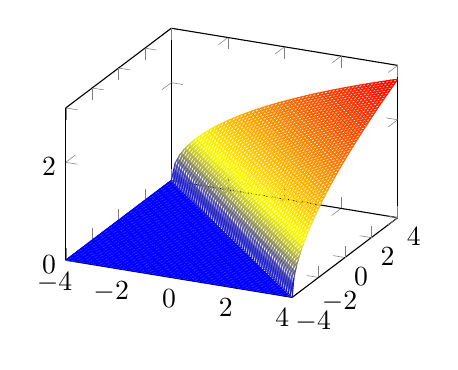
\begin{tikzpicture} 
%	\begin{axis}[
%			height=5cm,xlabel=$x$, ylabel=$y$, zlabel=$z$,zmin=0] 
%		\addplot3[surf,shader=flat,opacity=.8,samples=60] gnuplot {((x + y <0) && (x>3)) ?1/0}; 
%		%\addplot3[mesh,samples=60,domain=-4:4, y domain=-4:4]  {(sign(x+y)+1)/2*sqrt(abs(x+y))}; 
%		%\addplot3[white,surf,shader=interp,samples=50] {(x+y)sqrt(abs(x+y))}; 
%		%\filldraw[white] (axis cs:-4,-4,0) -- (axis cs:4,-4,0) -- (axis cs: -4,4,0); 
%\end{axis} 
	\begin{axis}[height=5cm,zmin=0]
		\addplot3[mesh,samples=60,domain=-4:4, y domain=-4:4]  {(sign(x+y)+1)/2*sqrt(abs(x+y))}; 
	\end{axis}
\end{tikzpicture}
